% s_fpga.tex -- final report, FPGA implementation and board results (P7--P10).
% Drop-in section for the report source of midterm_mtr-22/1_report_source (same preamble: \nb, newtext, \lvl, cleveref).
% Figure: figs/board.pdf (made by fpga/host/plot_board.py --report).  Numbers: fpga/FPGA_RESULTS.md and the logs it cites.
% Colour rule as in the mid-term report: black = planned in the PPR, blue = new results and calculations.
% Written with AI assistance (Claude, Anthropic), project decision D-06.

\section{FPGA Implementation and Board Results: P7--P10}
\label{sec:fpga}
The PPR planned a fully parallel datapath on the Boolean Board's XC7S50 \cite{realdigitalboard}, verified against the fixed-point model by automated comparison, synthesised at several word lengths and measured on the board with the three receivers running concurrently on one impaired stream (\cref{fig:system}). \nb{All four steps are done. The central result is that the board's counters are \emph{identical} to the bit-true model, not merely close: for eight configurations covering the FPGA step sizes, the variation rates and both channels, every error count, squared-error sum and stall count measured on the board equals the \lvl{L2} value (\lvl{L5} $=$ \lvl{L2}). The \lvl{L2} word-length study of \cref{sec:fxp} therefore also describes this hardware, and the board measurements below are measurements of the designed system, not of an approximation to it.}

\subsection{Architecture (P7)}
\label{sec:fpgaarch}
\begin{newtext}
\noindent\textbf{Symbol timing.} The noise generator (12 LFSRs, sum of uniforms \cite{alfke1996,irwin1927,hall1927}) needs 16 shift steps per sample, so one symbol is processed every 16 clocks: 6.25\,Msymbol/s at 100\,MHz, about $2\times10^7$ evaluated bits in 3\,s of board time. Within a symbol (\cref{fig:fpgatiming}) the front end forms $r[n]$ in two clocks and the LMS core works for ten: coefficients from the accumulators, the 32 filter products, a two-level adder tree, $y$, $e$, the 16 update products, the $\mu$ shift, a limiter, and the accumulator write. The update of symbol $n$ is in the accumulators before symbol $n+1$ starts, so the hardware runs the plain LMS recursion with no adaptation delay ($D=0$); registers were added only \emph{inside} the symbol period, which leaves the algorithm unchanged, never across symbols, which would make it delayed LMS \cite{long1989}. A testbench check enforces this budget; as a negative control, symbols 9 clocks apart are flagged and 3979 of 4000 outputs then differ.

\noindent\textbf{Arithmetic.} The formats of \cref{tab:formats} are kept exactly. Each product is at most $16\times16$ bits and maps to one DSP48E1 \cite{xilinxug479}; the rounding constant of the update is added in the post-adder of the update multiplier, so round-to-nearest costs no extra DSP. The channel FIR needs no multiplier: its taps are $\pm1$, $\pm512c$ (a shifted 7-bit counter) and a constant. $\mu=2^{-p}$ is a run-time input (a shift), $B_{\rm mul}$, $B_{\rm acc}$ and the rounding rule are synthesis parameters.

\noindent\textbf{Board operation.} In \emph{host mode} the PC sends a complete experiment over the USB-UART (step size, rate, channel limits, noise level, training length, run length, payload seed and the twelve 36-bit noise seeds) and receives all counters with a checksum when the run ends; this is how the \lvl{L5} results were measured. Payload bits come from an on-chip LFSR ($x^{31}+x^{28}+1$) that the PC regenerates exactly, which is what makes a count-for-count comparison possible. In \emph{demo mode} the switches select the rate, $\mu$, Eb/N0 and channel, and the two seven-segment displays show the R2 (or R1) and R3 error counts per window of $2^{20}$ tracking symbols, so the examiner can raise the variation rate and watch R3 lose accuracy while R2 is unaffected.
\end{newtext}

\begin{figure}[t]
\centering
\begin{tikzpicture}[x=0.42cm,y=0.5cm,font=\scriptsize]
  \foreach \i in {1,...,16} { \draw[gray!60] (\i-1,0) rectangle (\i,0.6); \node at (\i-0.5,0.3) {\i}; }
  \node[anchor=east] at (-0.2,0.3) {clock};
  \draw[fill=gray!25] (0,-0.9) rectangle (16,-0.3); \node at (8,-0.6) {next noise word: 16 LFSR steps};
  \draw[fill=blue!10] (0,-1.8) rectangle (1,-1.2);  \node at (0.5,-1.5) {n};
  \draw[fill=blue!20] (1,-1.8) rectangle (3,-1.2);  \node at (2,-1.5) {front};
  \draw[fill=blue!35] (3,-1.8) rectangle (13,-1.2); \node at (8,-1.5) {LMS (10 clocks)};
  \draw[fill=blue!20] (13,-1.8) rectangle (14,-1.2); \node at (13.5,-1.5) {cnt};
  \node at (15,-1.5) {spare};
  \draw[-{Latex}] (13,-2.2) -- (13,-1.85); \node[anchor=north] at (13,-2.2) {update written};
  \draw[-{Latex}] (16,-2.75) -- (16,-1.85); \node[anchor=north east] at (16.3,-2.75) {next symbol};
\end{tikzpicture}
\caption{\nb{Processing of one symbol in hardware (\lvl{L3}). n: noise sample latched; front: channel, noise and rounding to s16.12; LMS: coefficients from the accumulators, 32 filter products, two adder levels, $y$, $e$, 16 update products, $\mu$ shift, limiter, accumulator write (one clock each); cnt: error and squared-error counters. The update is complete before the next symbol starts, so the adaptation is plain LMS ($D=0$).}}
\label{fig:fpgatiming}
\end{figure}

\subsection{RTL verification (P8, \lvl{L3})}
\label{sec:fpgaver}
\nb{The behavioural mid-term RTL was rewritten for synthesis with the arithmetic unchanged; its noise generator and PRBS were synthesisable and are used as they were. Every comparison is automated against the \lvl{L2} functions of the mid-term (\cref{tab:fpgaver}); none relies on waveform inspection. Mismatches anywhere in a per-symbol signal or a counter fail a test.}

\begin{table}[t]
\centering
\footnotesize
\begin{tabular}{@{}p{2.0cm}p{3.8cm}l@{}}
\toprule
Test & Coverage & Result\\
\midrule
LMS core & 13 cases: $B_{\rm acc}$ 10--32, $B_{\rm mul}$ 8--16, $\mu=2^{-2}$--$2^{-11}$, truncation, saturation, $N_T=30000$ & identical\\
Cycle budget & 10 clocks per symbol; 9 clocks (negative control) & pass; flagged\\
Vendor simulator & Vivado xsim, 3 cases & identical\\
Full chain & 13 cases: mid-term A--G, $B_{\rm acc}$ 26/32, $\mu$ ends, $N_T=30000$, payload LFSR & identical\\
Top level & two experiments as UART command frames & identical\\
\bottomrule
\end{tabular}
\caption{\nb{Bit-exact verification against the bit-true model (\lvl{L3}, iverilog unless stated). ``Identical'': every per-symbol value ($r$, $d$, $y$, $e$ of R2 and R3) and every counter equal to \lvl{L2}.}}
\label{tab:fpgaver}
\end{table}

\subsection{Synthesis and timing (P9, \lvl{L4})}
\label{sec:fpgasyn}
\nb{The complete design (receivers, noise, UART, board controls) was placed and routed with Vivado~2025.2 at 100\,MHz (\cref{tab:fpgares}). It uses 51 of 120 DSP48E1, against the PPR's estimate of 51 for the datapath and $\approx$54 with the counters: 48 in the two adaptive and frozen filters and the update, one for $\sigma\cdot$noise and two for the squared errors; the channel needs none. Timing is met with positive slack in both builds; the critical path of the 16-bit build is the noise generator's 12-word adder, not the LMS loop. The estimated $F_{\max}$ is $1/(10\,{\rm ns}-{\rm WNS})$, not a measurement at a higher clock.}

\begin{table}[t]
\centering
\footnotesize
\setlength{\tabcolsep}{4.5pt}
\begin{tabular}{@{}lrrrrrr@{}}
\toprule
Build & DSP & LUT & FF & WNS & $F_{\max}$ & Power\\
\midrule
$B_{\rm acc}=16$ & 51 & 4825 & 4670 & $+0.30$\,ns & 103\,MHz & 0.14\,W\\
$B_{\rm acc}=26$ & 51 & 4851 & 4988 & $+0.72$\,ns & 108\,MHz & 0.14\,W\\
\midrule
\multicolumn{7}{@{}l}{\emph{LMS core alone, $B_{\rm mul}=12$ (out of context)}}\\
$B_{\rm acc}=12$ & 48 & 2817 & 1515 & $+1.62$\,ns & & \\
$B_{\rm acc}=14$ & 48 & 2942 & 1579 & $+1.59$\,ns & & \\
$B_{\rm acc}=16$ & 48 & 3009 & 1643 & $+1.67$\,ns & & \\
$B_{\rm acc}=26$ & 48 & 3068 & 1962 & $+1.86$\,ns & & \\
$B_{\rm acc}=32$ & 48 & 5080 & 2290 & $+0.97$\,ns & & \\
\bottomrule
\end{tabular}
\caption{\nb{Resources and timing after routing on the XC7S50 (120 DSP48E1, 32\,600 LUT, 65\,200 FF), $B_{\rm mul}=12$, round to nearest (\lvl{L4}). Top: complete design; no block RAM. Bottom: the LMS core alone; $B_{\rm mul}=8$ and 16 give the same DSP and FF counts and LUT counts within 82 of these. Power is Vivado's estimate.}}
\label{tab:fpgares}
\end{table}

\nb{\emph{Hardware cost of word length.} (1)~The DSP count is flat at 48 for every $B_{\rm mul}\in\{8,12,16\}$ and $B_{\rm acc}\in\{12,\dots,32\}$, because every product fits one $25\times18$ multiplier. (2)~Flip-flops grow by 32 per accumulator bit (16 accumulators and their update registers). (3)~LUTs are nearly flat up to 26 bits and rise by $\approx$2000 at 32 bits, where the update word no longer fits the DSP post-adder path. (4)~The multiplier width costs nothing measurable. Combined with \cref{sec:fxp}, which found that $B_{\rm acc}\ge16$ with rounding preserves $S^\star_{\rm MSE}$ at all seven FPGA step sizes, the cheapest configuration that preserves tracking is $B_{\rm mul}=12$, $B_{\rm acc}=16$, round to nearest; the 26-bit baseline costs 318 more flip-flops and 26 more LUTs in the complete design, and no DSP. Slack differences of a few hundred picoseconds between neighbouring widths are place-and-route variation, not a trend.}

\subsection{Board measurements (P10, \lvl{L5})}
\label{sec:board}
\nb{\emph{Board against model.} For each configuration of \cref{tab:board} the PC sent the seeds, the board ran $N_T=30000$ training symbols and the tracking part, and the PC ran the \lvl{L2} model on the same inputs. All eight counters (symbols, three error counts, two squared-error sums, stalls, updates) agree in every run, for both $B_{\rm acc}=16$ and 26, over 3.4 million symbols per build. This is the strongest available test of the implemented netlist: a single wrong bit anywhere in the datapath would change the squared-error sums.}

\begin{table}[t]
\centering
\footnotesize
\setlength{\tabcolsep}{3.5pt}
\begin{tabular}{@{}rrlrrr@{}}
\toprule
$\mu$ & $S$ & channel, Eb/N0 & symbols & errors R1/R2/R3 & $=$\lvl{L2}\\
\midrule
$2^{-8}$ & 28 & primary, 10\,dB & 400k & 18112/2534/230 & yes\\
$2^{-8}$ & 1000 & primary, 10\,dB & 400k & 17108/2831/122 & yes\\
$2^{-8}$ & 5 & primary, 10\,dB & 400k & 18267/2969/518 & yes\\
$2^{-5}$ & 1 & primary, 8\,dB & 300k & 17602/2682/9696 & yes\\
$2^{-11}$ & 224 & primary, 12\,dB & 300k & 10043/883/10 & yes\\
$2^{-8}$ & static & primary, 10\,dB & 300k & 274/1/3 & yes\\
$2^{-8}$ & 50 & control, 14\,dB & 300k & 134/1/0 & yes\\
$2^{-6}$ & 112 & primary, 6\,dB & 1000k & 82619/33928/21144 & yes\\
\bottomrule
\end{tabular}
\caption{\nb{Board counters against the bit-true model (\lvl{L5} vs \lvl{L2}), $B_{\rm mul}=12$, $B_{\rm acc}=16$, rounding, supervised; errors counted over the tracking part (symbols minus $N_T$). ``Yes'': all eight counters identical; the same holds for $B_{\rm acc}=26$ (error counts differ slightly from these because the arithmetic differs).}}
\label{tab:board}
\end{table}

\begin{figure*}[t]
\centering
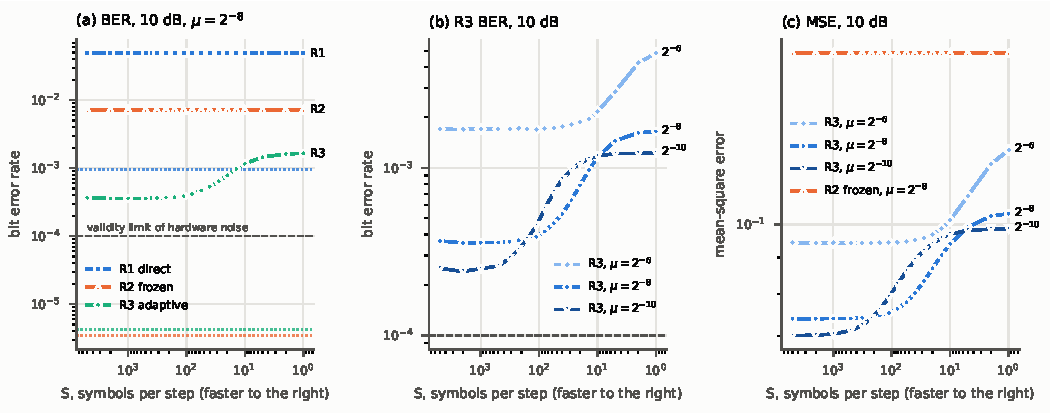
\includegraphics[width=\linewidth]{figs/board.pdf}
\caption{\nb{Tracking measured on the Boolean Board (\lvl{L5}): primary channel, $B_{\rm mul}=12$, $B_{\rm acc}=16$, rounding, supervised, LFSR sum-of-uniforms noise, one noise seed, $\approx2\times10^7$ bits per point over whole triangle periods. (a)~BER of R1, R2, R3 at 10\,dB, $\mu=2^{-8}$; dotted: static channel at $c=40$. (b)~R3 BER for $\mu=2^{-6}$, $2^{-8}$, $2^{-10}$. (c)~MSE of R3 for the three step sizes and of R2. Dashed: the $10^{-4}$ validity limit of the bounded hardware noise; BER below it is not claimed.}}
\label{fig:board}
\end{figure*}

\nb{\emph{Tracking on the board} (\cref{fig:board}). (1)~R1 and R2 do not depend on the variation rate (BER $4.9\times10^{-2}$ and $7.1\times10^{-3}$ at 10\,dB), as in \lvl{L1}: every window holds whole periods of the trajectory, and a receiver that does not adapt cannot notice speed. (2)~R3 is better than R2 at every rate, by a factor of 20 for slow variation and 4 at $S=1$ ($\mu=2^{-8}$): no $S_{\rm cross}$ within the grid, as in \cref{sec:p3}. (3)~R3's BER rises 15\,\% above its slow-variation level at about $S=320$, 80 and 14 for $\mu=2^{-10}$, $2^{-8}$ and $2^{-6}$: each factor of four in $\mu$ moves the onset by about a factor of four in $S$, the ordering of the \lvl{L1} boundaries (\cref{tab:sstar}). (4)~Which step size is best depends on the rate: $2^{-10}$ for $S\ge224$ (least gradient noise), $2^{-8}$ for $112\ge S\ge14$ (it follows, $2^{-10}$ lags), and $2^{-10}$ again for $S\le5$, where neither follows and the smaller step stays closer to the best fixed filter for the averaged channel. This is the tracking--step-size trade-off, measured in hardware. These are single-seed measurements; no boundary $S^\star$ is derived from them, because the project's criteria need the seed statistics of \lvl{L1}. They confirm the trend on the hardware; they do not replace the \lvl{L1} boundary.}

\nb{\emph{Accumulator width on the board.} With $B_{\rm acc}=16$, 6.6\,\% ($\mu=2^{-8}$) to 20\,\% ($\mu=2^{-10}$) of all nonzero coefficient updates round to zero, against 0.006\,\% and 0.03\,\% with 26 bits. Yet R3's BER and MSE agree between the two builds to three or four significant digits at every rate (e.g.\ $\mu=2^{-10}$, $S=28$: BER $9.77\times10^{-4}$ and $9.78\times10^{-4}$, MSE 0.0920 in both). With round-to-nearest the channel noise dithers the lost updates, as predicted by the stall analysis of \cref{sec:fxp}. On this hardware, then, update underflow is frequent but does not restrict tracking in the approved range; the PPR's hypothesis would need narrower accumulators, truncation or smaller step sizes to show.}

\noindent\textbf{Engineering significance.} \nb{(i)~The design question of the PPR, which precision and what hardware a given tracking rate needs, has a measured answer: a 12-bit multiplier word and a 16-bit accumulator with round-to-nearest track as well as the 26-bit baseline, cost 51 DSP slices and about 4.8k LUTs, and close timing at 100\,MHz without delayed LMS. (ii)~Because the board equals the model, the step-size and word-length conclusions of \cref{sec:results14,sec:fxp} carry over to the hardware for these configurations without a separate hardware sweep. (iii)~The DSP budget is set by the number of taps and receivers, not by word length; word length is paid for in flip-flops and, above 26 bits, LUTs.}

\noindent\textbf{Limits.} \nb{Hardware BER is quoted only down to about $10^{-4}$ (bounded noise). The board sweeps use one seed. Supervised adaptation only; decision-directed operation, NLMS and payload transport of audio and images over the UART were not implemented on the board. The bitstream is loaded over JTAG at each power-up. The RTL was written with AI assistance \cite{claude} and reviewed, executed and tested by the team; each module names the team member responsible for it.}
